From the experimental results in subsection \ref{subsec: Result and Analysis}, when there is enough information, the level set method can achieve a precise segmentation result. However, when the scene of the picture is more complex, the level set method cannot achieve the desired segmentation result. Therefore, some \textbf{pattern recognition} methods are proposed to bring more information about the target. For example, the regions of the target, and the probability that each pixel belongs to the target category. In the process of the contour evolution, the level set method relies on the statistic of pixels inside and outside the contour with fixed $\phi$ at this time, such as the mean, the weighted mean and the probability model about regions \cite{LevelSet:Discussion:lin2005probability}. And the level set method is more like an integration method of the information, which uses the energy functional minimization principle to construct a potential function. Moreover, this potential function can be set as the probability function, which is disposed by probabilities and Bayesian methods.

The GAT is used to find the optimal affine transformation of the standard prior shape based on the probability map. But it is based on the contour, and the probability map expresses the regions. Therefore, when the results of FCNs are poor, the GAT will fail to match. The failure result of the GAT is shown in Fig. \ref{fig: The failure result of the GAT}.
\begin{figure}[h]
    \centering
    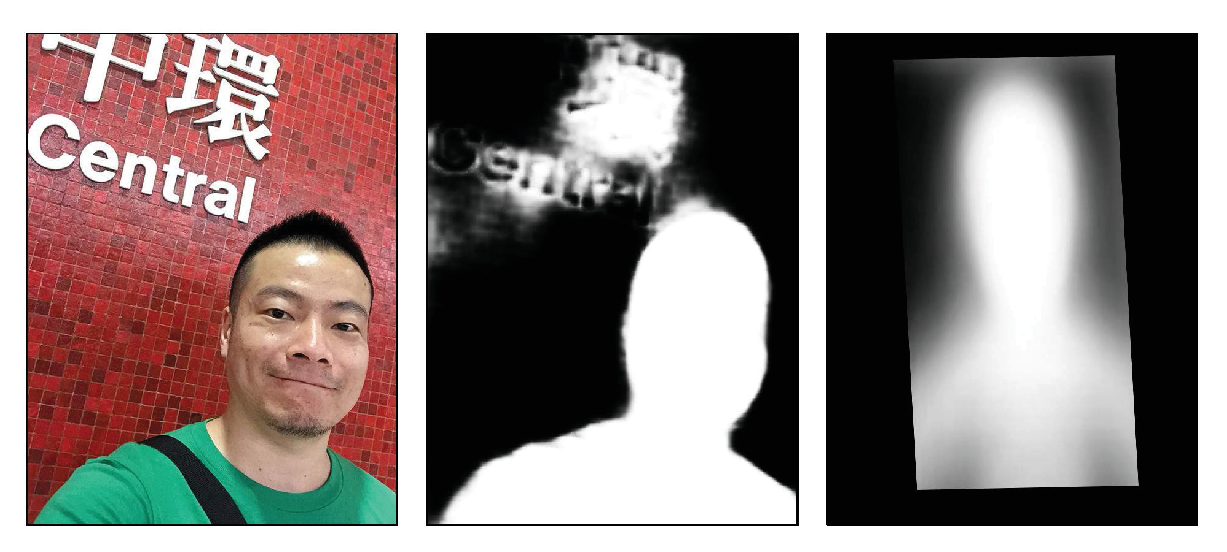
\includegraphics[width=7cm]{figs/GAT_Failed.eps}
    \caption{The failure result of the GAT.}
    \label{fig: The failure result of the GAT}
\end{figure}

Even if the pixels are very similar, the imprecise probability map and the corrected prior shape still have a large effect, causing that similar pixels are split apart. But we can draw on the idea of superpixels \cite{LevelSet:superpixels:achanta2012slic}. Most of those methods about the image segmentation can be summarized as how to extract and use the information in images. Therefore the most important issue is to build the dynamic hierarchical structured representation of images.
